\begin{figure}[t]
\center
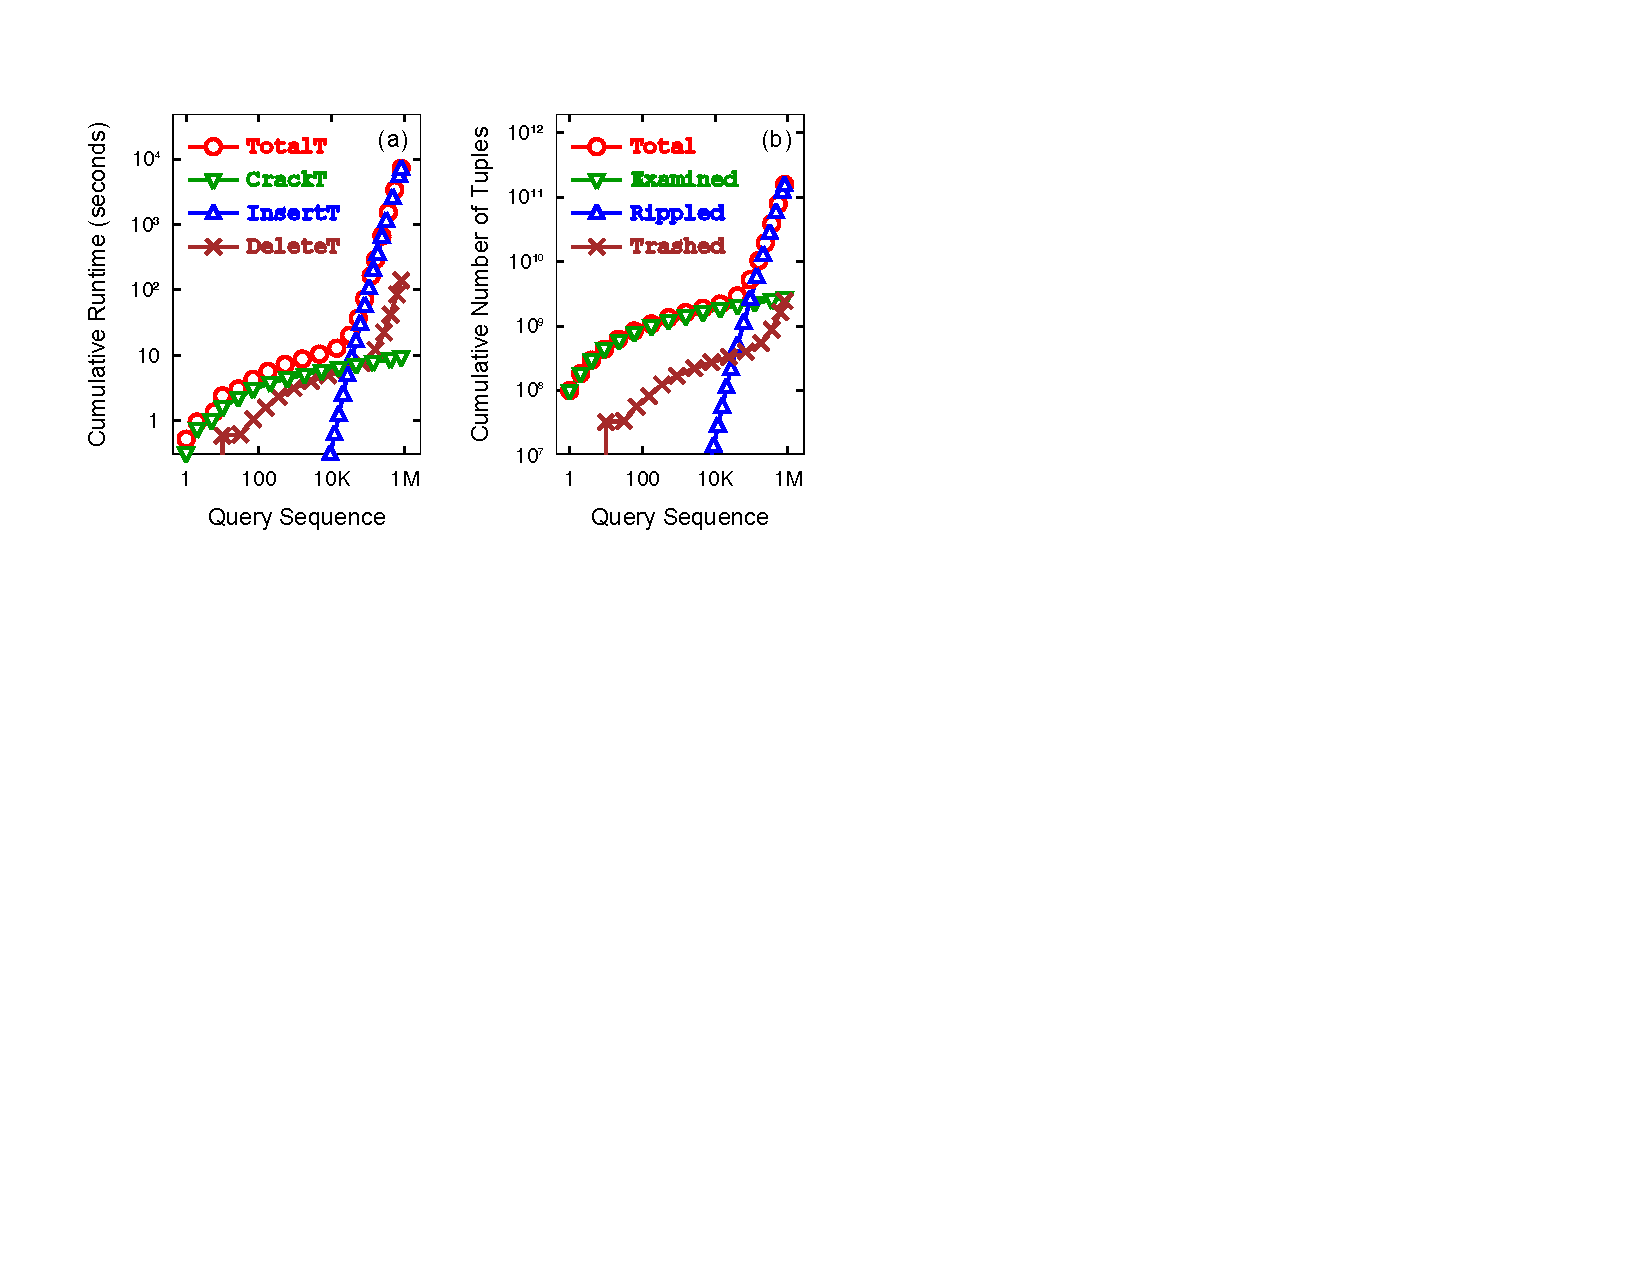
\includegraphics[width=.9\columnwidth]{graphs/figure4.pdf}
\vspace{-1em}
\caption{Non-resilience of adaptive indexing during long sequences of data injections interleaved with queries.}
\vspace{-1em}
\label{F:UpdatesProblem}
\end{figure}
\section{Resilient Adaptive Indexing}
\label{sec:cracke}

We showed in the previous section that while current adaptive indexing brings some significant advantages,
when it comes to long exploratory query sequences, especially when those are interleaved with updates,
then adaptive indexing loses all its performance advantages.
To deal with modern exploratory applications, we need adaptive indexing techniques which are resilient
to such problems and can maintain their adaptive properties in the long term.
In this section, we study the space of possible solutions and we propose Comb (Cracking Over Malleable Buckets), a new 
adaptive indexing technique that maintains all the desirable properties of current approaches,
while it is also resilient to cope with the data deluge challenges. 


\subsection{Target Performance}

Our goal is to maintain the main properties of existing adaptive indexing techniques
both {\em early} in a query sequence and as the query sequence {\em evolves}.
In this way, our target performance includes the following characteristics.
\begin{itemize}
\item \textbf{Lightweight}. The per query cost should be kept low, i.e., individual queries should not be penalized.
\vspace{-.5em}%
\item \textbf{Adaptive}. The system should be able to rapidly adjust to workload patterns.
\vspace{-.5em}%
\item \textbf{Resilient}. Performance should not degrade in the long run and all adaptive properties should be maintained.
\end{itemize}

\subsection{The Source of the Problem}

We can attribute the non-resilience problem of existing adaptive indexing techniques to
the maintenance and handling costs of the growing index structure
and of the dense array data structures.
As we have shown in Section \ref{sec:problem}, as query sequences evolve, 
the information stored in the index grows and it becomes much harder to maintain and traverse. 
The tree structure holding information regarding value ranges and piece boundaries grows with every 
query that  refines the index. Thus, as the query sequence grows, the tree grows as well and its traversal
leads to random memory access. In addition, in order to maintain the dense structure  of columns
and the partitioning information, 
merging of updates results in tuples being shuffled around.
The more the pieces in a cracking column, i.e., the more the information in the index, the more tuple
movements we have to do in order to put new values in or in order to move holes caused by deletions outside a given range.  

In order to deal with the non-resilience problem, we need to contain these extra costs, i.e., allow for
less expensive traversal of the tree part of the index and more efficient merging of updates.

\begin{figure*}[t]
\hspace{-3.5em}%
\Fig[b]{.5\columnwidth}{%
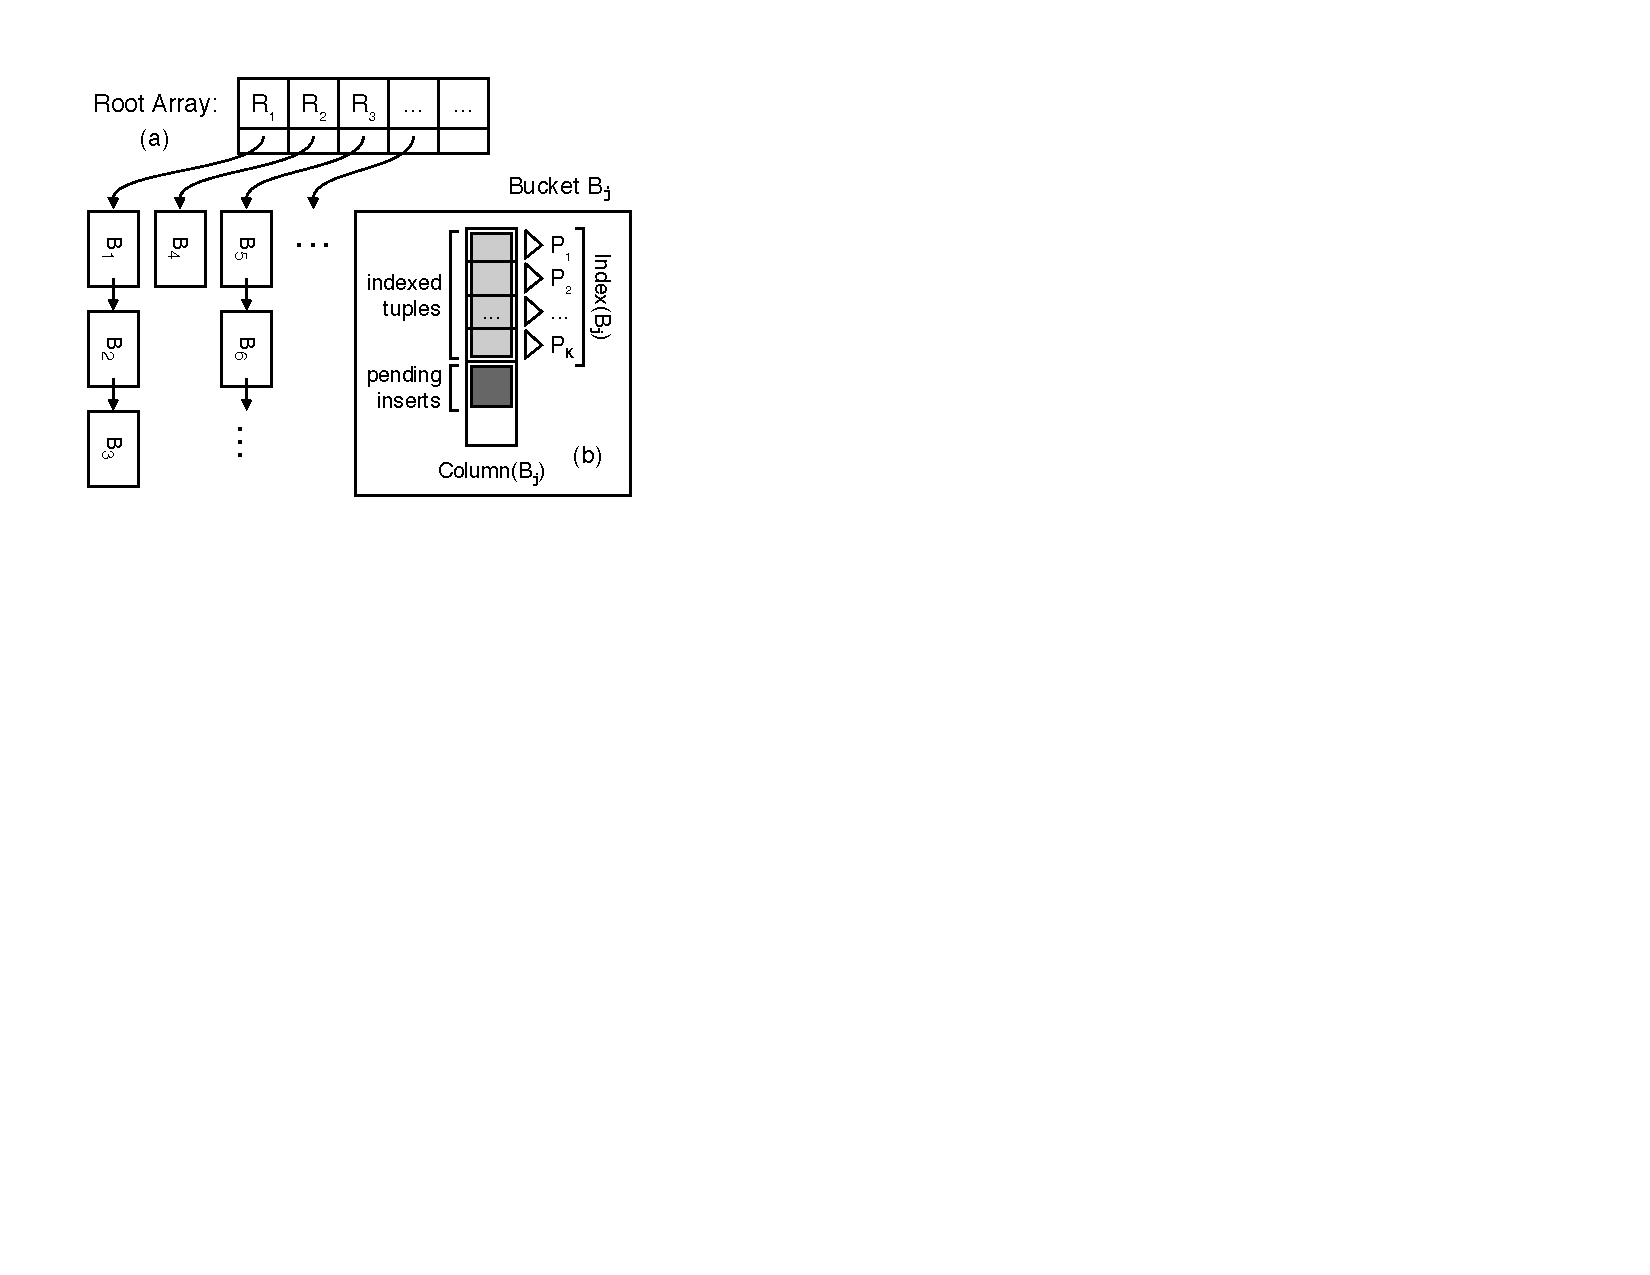
\includegraphics[width=1\columnwidth]{graphs/fig_crake.pdf}
\vspace{-1em}
\caption{The Comb structure.}
\vspace{-1em}
\label{F:crake}
}
\hfill
\hspace{-11.5em}%
\Fig[b]{.6\columnwidth}{%
\hspace{-.5em}%
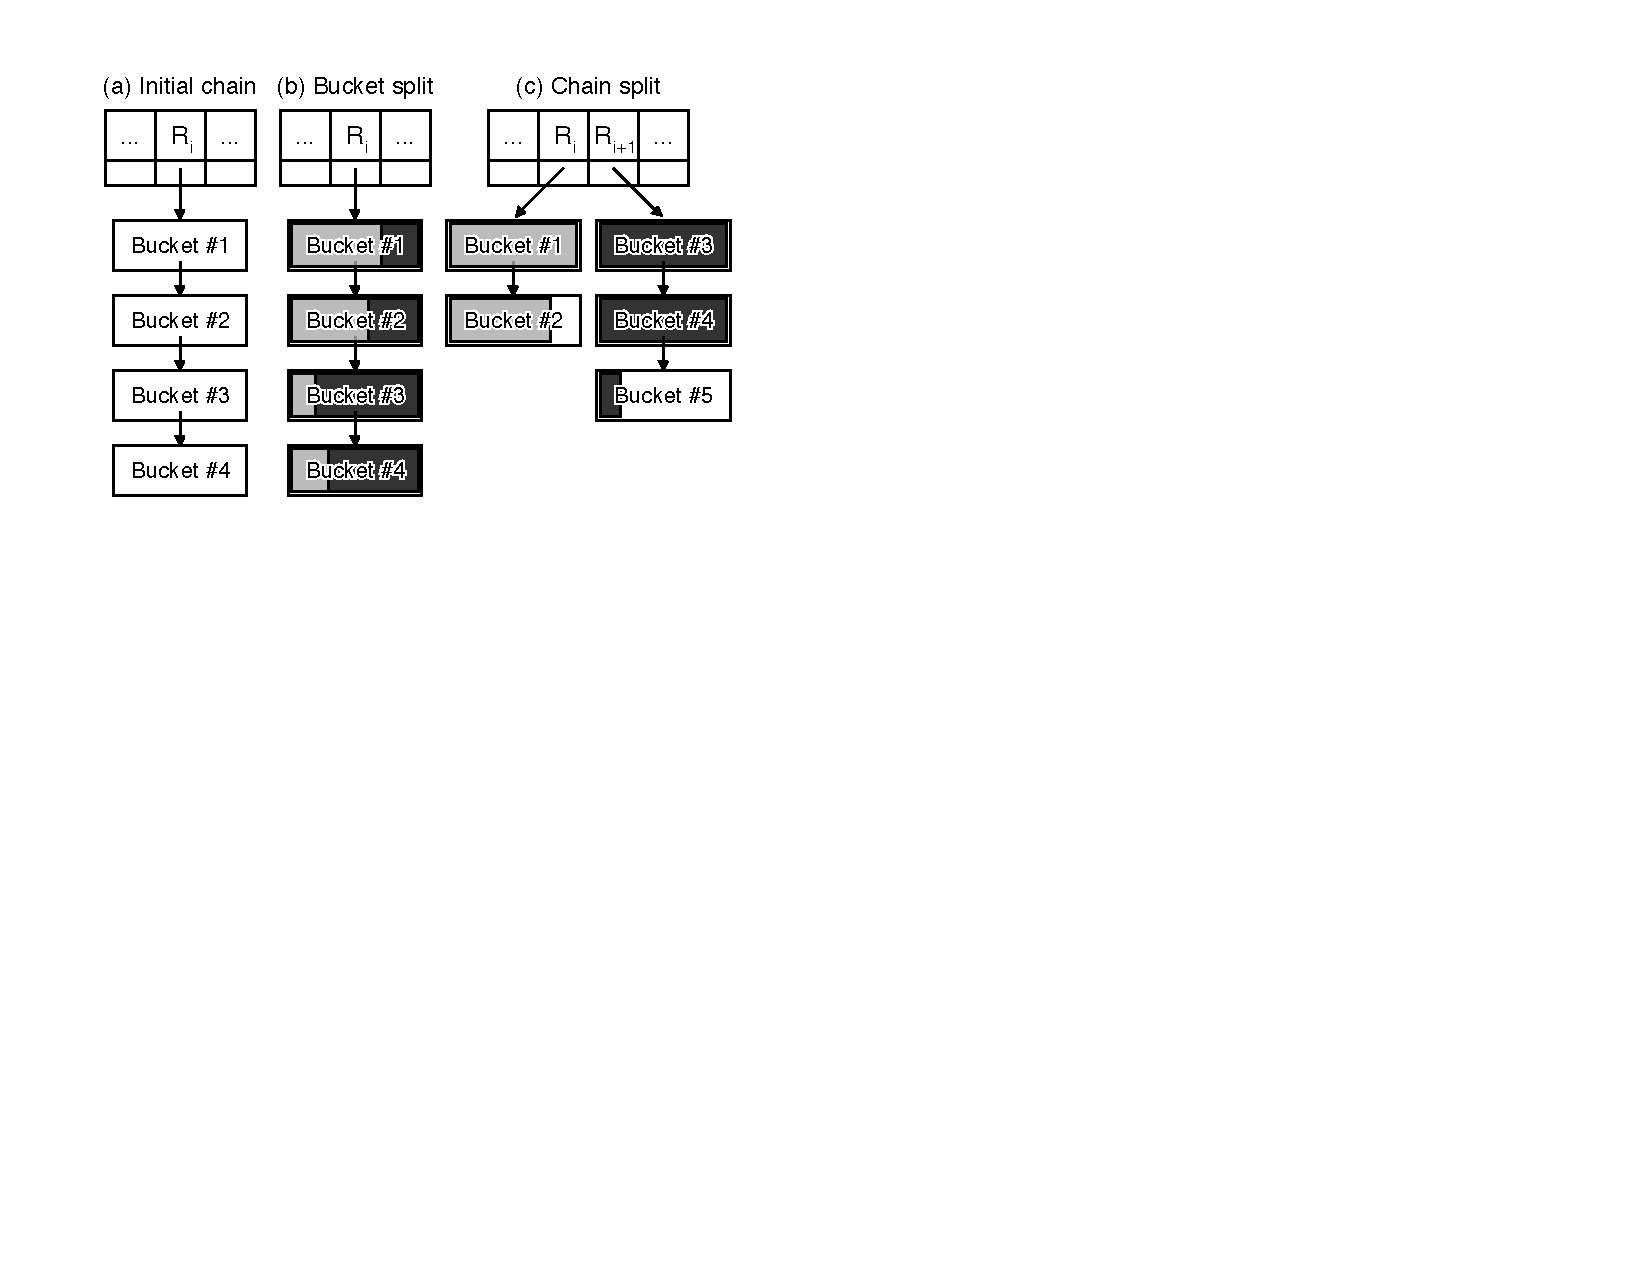
\includegraphics[width=1.05\columnwidth]{graphs/fig_crake_lazy.pdf}
\vspace{-1em}
\caption{Bucket chains and splits.}
\vspace{-1em}
\label{F:lazycrake}
}
\hfill
\hspace{-6.5em}%
\Fig[b]{.5\columnwidth}{%
\hspace{-6em}%
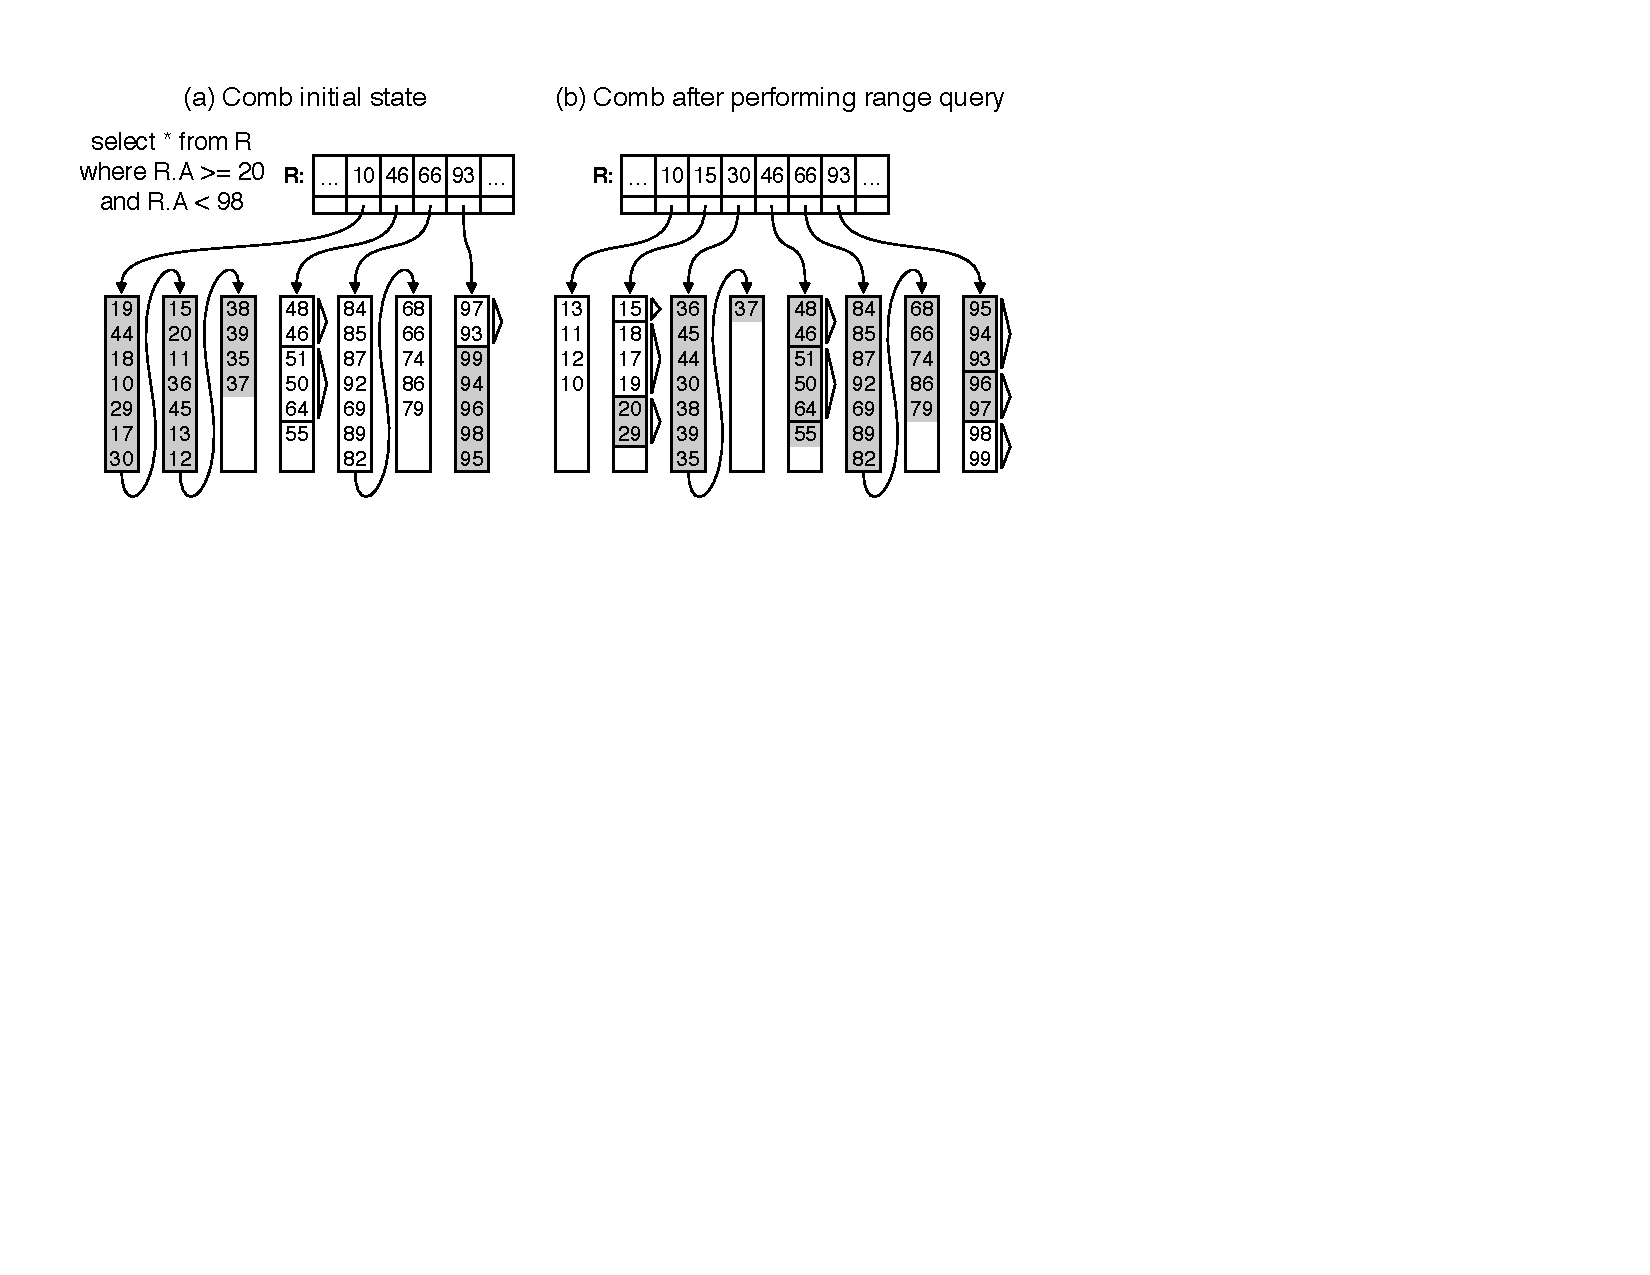
\includegraphics[width=1.8\columnwidth]{graphs/range_query.pdf}
\vspace{-1em}
\caption{Query example.}
\vspace{-1em}
\label{F:rangequery}
}
\end{figure*}

\subsection{Optimizing Existing Adaptive Indexing}
\label{sec:simple}

One way to deal with the non-resilience  problem of adaptive indexing is to patch existing 
adaptive indexing techniques so that they are less prone to performance degradation in long 
query sequences. One intuition is to restrict the growth of the index. 
By allowing the index to grow up to a certain size, and thus the column to be cracked up to a maximum number of pieces,
then there is a maximum traversal cost
as there is a maximum index depth for the tree part of the cracking index.
In addition, there is a maximum number of movements we have to do in order to 
update a cracking piece, as there is a maximum number of pieces (there are fewer pieces and thus bigger in size).
Below we introduce four directions on how to restrict the index size. 

\textbf{Crack-NoIndex.} This first approach allows cracking to continue working as normal with the exception 
that if a piece in the index  has reached a minimum size of $P_{min}$ tuples, then future queries continue to crack this
piece but do not inject this information in the tree part of the index.
The current query is answered as normal  but its refinements are not marked in the index and thus
cannot be exploited by future queries nor create excessive administration overheads.  

\textbf{Crack-Scan.} The next variation of cracking does not crack any more pieces 
in the column which reach  the threshold of $P_{min}$ tuples.
Instead, it scans a piece that it would normally crack.
As discussed in Section \ref{sec:problem}, a cracking range-select operator 
needs to touch at most two pieces at the edges of its target range. 
Thus, these extra scan actions add only a limited cost.
Contrary to the Crack-NoIndex approach,
Crack-Scan cannot return a view of the whole result and needs to materialize the qualifying values of the edge pieces.

\textbf{Crack-Sort.} The third alternative aims towards maximum read performance. 
When the piece size limit is reached, then a future query sorts completely a piece which should have been normally cracked.
The information that this piece is sorted is maintained in the tree index (an extra bit)
and future queries may simply binary search when their boundaries fall within this piece.

\textbf{Crack-Forget.} Finally, another interesting direction is to continue cracking as normal
with the addition that we ``forget" part of the indexing information in an adaptive way.
We can drop some of the partitioning knowledge only when necessary; this results in less pieces and thus less 
administrative overhead and update costs. In particular, in the spirit of adaptive indexing, 
we can drop pieces which are about to be updated and thus create extra costs.
This action is performed directly in the select operator during processing of a query that needs those pieces
and only if we exceed a maximum number of pieces in the index. With this strategy the index continuously adapts 
via cracking and still is able to avoid expensive updates in very well refined areas of the index.


\subsection{Comb: Cracking Over Malleable Buckets}
Optimizations and fine-grain variants of existing adaptive indexing techniques are limited
by fundamental choices in the original approaches. 
In Section \ref{sec:experiments}, we show that even though our optimized adaptive indexing designs
help with the resilience problem, the improvement is not enough.
% , still though there is potential to achieve significantly better performance.

\textbf{Comb.}
In this section, we introduce Comb (Cracking Over Malleable Buckets),
a novel adaptive indexing technique designed and tailored
to deal with the non-resilience problem of adaptive indexing when it comes to long strings of read and write queries,
while still maintaining all the good properties of previous adaptive indexing approaches.



A high level view of the Comb structure is shown in Figure \ref{F:crake}.
There are two fundamental components; (a) the root array and (b) the buckets.
A single Comb structure $Comb(C)$ maintains the contents of a single column $C$ in a column-store. 

\textbf{Root Array.}
The buckets in a Comb structure contain the actual tuples, while the root array serves the role
of guiding queries to the proper bucket.
As Figure \ref{F:crake} shows, each entry $R_i$ in the root array corresponds to a collection 
of one or more chained buckets $CB_i$.
Each root entry contains two variables. The first one is a physical pointer $Pointer(R_i)$
to the first bucket $B_i$ in chain $CB_i$.
The second one is the key $Key(R_i)$, which defines the starting point of the value range corresponding to bucket 
collection $CB_i$.
The root array is maintained sorted on its key values.

\textbf{Buckets.}
Each bucket in an index $Comb(C)$ is responsible for holding part of the tuples of the base column $C$.
Each chain of buckets $CB_i$, corresponding to root element $R_i$, holds all values in the range $[Key(R_i)$,$Key(R_{i+1}))$.
The value $Key(R_i)$ is the smallest value which is currently stored inside the buckets of $CB_i$.
The bottom part of Figure \ref{F:crake} shows how chains of malleable buckets 
connect to the root array and an instance of the internals of a bucket.

Inside each bucket $B_j$, there is a column, $Column(B_j)$, which holds the local tuples. 
This column is continuously cracked and reorganized as more queries arrive.
The last part of $Column(B_j)$ contains values which have been inserted but not yet merged with
the rest of the partitioned values in $Column(B_j)$.  

In addition, there is another array, $Index(B_j)$, which maintains the partitioning information for $Column(B_j)$;
it contains the pivots used for cracking on $Column(B_j)$ and the corresponding physical position
where each piece starts in $Column(B_j)$; it is equivalent to the root array with the difference that it is used 
for guiding through the local column. 
Array $Index(B_j)$ is maintained sorted.

Furthermore, there is a bit vector, $Sorted(B_j)$, which is aligned to $Index(B_j)$ and 
maintains information regarding whether a piece in $Column(B_j)$ is sorted or not (as in Crack-Sort). 

\textbf{Slicing.}
Comb carefully slices the data and the indexing information across buckets
and across the pieces in the local columns within each bucket.
The main target is to minimize the administrative costs as well as the access and update costs.

In a column of $N$ total tuples, each bucket may contain up to a maximum of $M$ tuples. 
In our experimental evaluation we found that performance is best when $M$ is such that each bucket fits in L1 cache.
Inside each bucket, each local column may be partitioned up to a maximum number of pieces $P$. 
By default, this is purposely kept small in the order of $P=128$ pieces per bucket to guarantee low update costs.
We will discuss the effect of those parameters later on.
In this way, the root array may contain up to $N/M$ entries, 
while each cracking piece in the local column inside each bucket contains on average  $M/P$ tuples. 

As we focus on main-memory environments, we design
Comb to have one root array for the following reason.
For example, consider a typical 2MB L2 cache; if the root array fits in L2,
our Comb implementation can index  
a raw column of 256GB integer values (including auxiliary row IDs).\footnote{
\small
When $N$ is even smaller,  a good choice is that of $M = sqrt(N)$,
balancing the size of the root array and buckets.
}
This is already more than conventional memory capacity and 
also more than the typical size of a single column in a database.
% Comb can already hold up to 
% If the root array fits in a typical 2MB L2-cache and we pick $M = sqrt(N)$, where $N$ is the size of indexed column $C$,
% then  Comb can hold up to $(2 MB)^2 ~= 512 GB$, 
% which is more than the conventional memory capacity and 
% also it is more than the typical size of a single column in a database.
Multi-level root arrays are certainly a possible extension.
However, this is beyond the scope of this paper.
% When $N$ is not so large as the above,
% a good choice of $M = sqrt(N)$ balancing the size of the root array
% and buckets.

\textbf{Insertions.}
Let us now discuss how new values are inserted in Comb.
Assume a new value $v$. 
Comb first searches its root array to find the bucket chain which contains $v$.
Since the root array is always sorted, searching is done via binary search and costs $O(\log(N/M))$.
The result bucket chain $CB_i$ is the one where $Key(CB_i)<=v<Key(CB_{i+1})$.
There are two cases when inserting a new value $v$. 

\textbf{Appending Inserts and Chaining Buckets.}
The first case is that the corresponding bucket chain $CB_i$ where $v$ belongs has enough space to accommodate $v$.
This means that the last bucket $B_j$ in $CB_i$ has at least one empty position.
In this case, the new value $v$ is simply appended at the pending inserts part of $Column(B_j)$.
This means that $v$ is placed immediately after the last indexed value of $Column(B_j)$ or immediately after the
last pending insert in the case that there are already pending inserts in $Column(B_j)$.
Holding both indexed values and pending inserts in $Column(B_j)$ means that a query which needs all values
in the value range stored in $B_j$ can blindly retrieve $Column(B_j)$. Analysis and merging is needed
only if a query needs to search within the range of $Column(B_j)$. 

The second case when inserting a value $v$ in a chain $CB_i$
is when the last bucket $B_j$ is full and no more values can be stored in $CB_i$.
In this case, Comb creates a new empty bucket $B_{new}$
and \emph{chains} $B_{new}$ to $B_j$. The new value is appended as a pending insert in $B_{new}$.
Examples of several buckets chained together are shown in Figures \ref{F:crake}, \ref{F:lazycrake} and \ref{F:rangequery}. 
All buckets under the same root entry $R_i$ contain values in $[Key(R_i),Key(R_{i+1}))$.

The design option to chain buckets under the same root entry guarantees low-cost insertions.
However, at the same time, the whole Comb structure should remain well adjusted to the workload to 
accommodate fast read access.
This means that there should be no individual long bucket chains in hot ranges.
Therefore, as we discuss later on, the buckets are {\em malleable}: 
queries can adaptively and on demand split chained buckets to balance
and optimize the value ranges which are relevant for the workload. 
An alternative design would be to eagerly split buckets during insertions.
However, we show in Section \ref{sec:experiments} that this is not a favorable design as it 
hurts the adaptive behavior of Comb. 



\textbf{Merging Inserts Inside a Bucket.}
Locally within each bucket $B_j$, insertions remain as pending insertions, stored at the last part of $Column(B_j)$
as shown in Figure \ref{F:crake}.
Insertions are merged with the indexed part of $Column(B_j)$ 
only when a query needs to refine the indexing information in $B_j$ or when deletes arrive in $B_j$. 
Comb merges local insertions in its cracked bucket columns using the cracking update algorithms 
as described in Section \ref{sec:problem} and in \cite{IKM:SIGMOD07}.
However, with Comb, the size of the columns as well as the partitioning depth of cracking in its local bucket 
columns are all kept under certain limits. This enables Comb to significantly restrict the update costs
by doing only small local actions within a single bucket when merging an update.
In addition, during query processing only the boundary pieces need to be updated;
we elaborate more on this important detail later in this section when we discuss about range queries.


\textbf{Initialization.}
Initializing a Comb index for an existing base column follows the procedure described for inserts above.
Starting with a single bucket, it continuously inserts new values and chains new buckets as they become full.
After loading a full column, and before any query has arrived,
the result is a multi-bucket structure as in Figure \ref{F:lazycrake}(a) with a single chain of buckets. 

\begin{figure}[t]
\begin{minipage}{4in}
{\small
\begin{tabbing}
16 16\= 16 \= 16 \= 16 \= 16 \= 16 \= 16 \= 16 \= 16 \= \kill
{\bf Algorithm} $\mathsf{RangeQuery}($low bound $v_1$, high bound $v_2)$\\
1.\>$lo$ = point\_query($v_1$)\\
2.\>$hi$ = point\_query($v_2$)\\
3.\>{\bf return} create\_view($lo$, $hi$) {\it// position of $v$ in Comb} \\
\\
{\bf function} $\mathsf{point\_query}($boundary value $v)$\\
4.\>{\bf if} (isEmpty($R$)) {\bf return} \{$|R|$, 0, 0\} {\it// past-the-end position}\\
5.\>$i$ = lower\_bound($R$, $v$) {\it// the first $i$ such that $Key(R_i) \geq v$}\\
6.\>$i$ = make\_standalone($i$, $v$)\\
7.\>$j$ = $Pointer(R_i)$\\
8.\>$k$ = crack($j$, $v$)\\
9.\>{\bf return} \{$i$, $j$, $k$\}\\
\\
{\bf function} $\mathsf{make\_standalone}($root index $i$, boundary value $v)$\\
10.\>{\bf while} (true) {\bf do}\\
11.\>\>$j$ = the first bucket pointed by $Pointer(R_i)$\\
12.\>\>{\bf if} ($B_j$ does not have a next bucket) {\bf break}\\
13.\>\>stochastic\_split\_chain($i$)\\
14.\>\>{\bf if} ($v \geq Key(R_{i+1}$)) $i = i+1$ {\it// adjust root index to where $v$ is}\\
15.\>{\bf return} $i$\\
\\
{\bf function} $\mathsf{stochastic\_split\_chain}($root index $i)$\\
16.\>$pv$ = pick\_random\_pivot(i) {\it// stochastic crack pivot value}\\
17.\>{\bf for} ($j$ = $|R|-1$; $j>i$; $j$-{}-) {\bf do} {\it// shift elements at $j > i$ to the right}\\
18.\>\>$Pointer(R_{i+1}) = Pointer(R_i)$\\
19.\>\>$Key(R_{i+1}) = Key(R_i)$\\
20.\>$|R|$ = $|R|+1$ {\it// increase the number of stored tuples |R|}\\
21.\>$Key(R_{i+1})$ = $pv$ {\it// set the smallest value in $R_{i+1}$ bucket chain}\\
22.\>perform split\_chain($i$, $pv$) which split a bucket chain pointed by\\
\>$Pointer(R_i)$, transferring tuples with values $\geq pv$ to buckets\\
\>in chain $R_{i+1}$ (implementation details are in Section \ref{sec:splitting})\\
\\
{\bf function} $\mathsf{crack}($bucket number $j$, boundary value $v)$\\
23.\>flush\_pending\_inserts($j$)\\
24.\>let $P_v$ = the (local) cracker piece of $B_j$ where $v$ is in\\
25.\>{\bf while} ($|P_v|$ > $CRACK\_AT$) stochastic\_split($P_v$) {\it// perform DD1R}\\
26.\>{\bf if} ($P_v$'s sorted flag is not set)\\
27.\>\>{\bf if} (this is a read query) sort the piece $P_v$ and set its sorted flag\\
28.\>\>{\bf else} {\bf return} the position of $v$ in $P_v$ via linear scan\\
29.\>{\bf return} the position of $v$ in $P_v$ via binary search\\
\\
{\bf function} $\mathsf{flush\_pending\_inserts}($bucket number $j)$\\
30.\>if (no local cracker index) consider all tuples are merged and {\bf return}\\
31.\>do merge insert completely to all the (local) pending tuples in $B_j$\\
32.\>unset the sorted flags of the pieces that are touched during merging\\
\end{tabbing}
}
\end{minipage}
\vspace{-1em}
\caption{Range query in Comb.}\label{algo:pointquery}
\vspace{-1.5em}
\end{figure}

% We define an iterator as a tuple with 3 values: \{$i$, $j$, $k$\}.
% An iterator is used to locate the position of a tuple.
% $i$ is the index of the root array, $j$ is the bucket number,
% and $k$ is the position of the tuple in the bucket $B_j$.

% $RangeQuery(v_1,v_2)$ returns a view consisting of an iterator such that positions before 
% the iterator is $<v$ and positions after the iterator is $\geq v$.
% The iterator is constructed by first finding the index of the root array ($i$)
% containing the tuple with value $v$ (line 2).
% The bucket pointed by the root array must be standalone (line 3)
% otherwise the bucket chain is split until it is standalone (line 8-11). 
% Next we retrieve the (standalone) bucket number ($j$) pointed by the root array (line 4).
% The bucket's array is then cracked on value $v$ and the cracked position is at $k$.
% We now have all the necessary ingredients to construct the pointer \{$i$, $j$, $k$\}.


\textbf{Deletes.}
For robustness reasons deletes follow an eager strategy and are applied 
in one go in each bucket. If we want to delete a value $v$, we first locate the
corresponding bucket $B_i$. Then, first all pending, if any, local inserts are merged
and subsequently we locate and delete $v$ by shuffling the tuple at the end of its
piece as described in Section \ref{sec:problem}.
In case there are several chained buckets under the same root entry,
then all chained buckets are updated.

An alternative strategy would be to allow deletes to remain pending and only merge them later on
as we do with inserts. However, as we show later on in Section \ref{sec:experiments}, 
this is not a robust solution as it can severely hurt read queries. 

\textbf{Continuous Adaptation.}
Comb is an adaptive index. As such queries are the driving force which shapes the index.
As more queries arrive, the index is continuously refined to adjust to the workload patterns.
The more a value range is queried, the more resolution the index adopts in this range.
At the same time, value ranges not queried are seen in a much more coarse resolution until relevant queries arrive.

\textbf{Adaptation During Queries.}
We now proceed to describe how select operations work  on top of Comb.
Figures \ref{F:lazycrake} and \ref{F:rangequery}  show how Comb is adaptively refined after a read query.
Figure \ref{F:lazycrake} shows how a single chain is split into two new ones,
while Figure \ref{F:rangequery} shows the end result of a full range query after all its split and cracking actions.
The chains at the borders of the requested range are adaptively split, while the buckets
at the very borders are cracked using the query bounds. 
This way, Comb adapts both at a global level by splitting chains at hot workload areas
and at a local level by refining the index information within buckets in hot areas.
The work performed is minimized as only the 2 boundary chain buckets need to be touched, i.e., the chains where the query bounds fall;
all chains and buckets in between are known to qualify so there is no need to be refined 
(this is similar to the discussion we did for cracking 
in Figure \ref{F:CrackExample} and Section \ref{sec:problem}).
Given that we do not have to refine all chains in between the query boundaries, 
this also means that we do not have to merge local updates in their respective buckets 
as we need all qualifying values anyway (both indexed and non-indexed values).
This is why a more lazy approach to inserts is beneficial.
With deletes, however, we need to guarantee there are no deletes leftover across all qualifying buckets
both in the borders of the queried range and in between. Being lazy creates excessive costs at query time, hence,
we choose eager deletes locally within each bucket.
We revisit the last two points in Section \ref{sec:experiments}. 


\textbf{Querying Comb.}
The algorithm for a Comb range select is described in detail Algorithm \ref{algo:pointquery}.
%In our pseudocode presentation, array indexing is also denoted by subscripts, e.g.
%$R[i]$ by $R_i$ (line 7),
%and $|x|$ is the size of array $x$, so $|R| = |R| + 1$ increases the array $R$ by 1.
Assume a select operator requesting all values in $[low,high]$ from column $C$.
Comb first searches its root array to find the bucket chain $CB_{low}$ 
which contains $low$ and the chain $CB_{high}$ which contains $high$.
Since the root array is always sorted, searching is done via binary search and costs $O(\log(N/M)$.

For ease of presentation, assume first that both boundary chains contain one bucket each. 
For chain $CB_{low}$, the select operator searches within the single bucket $B_{low}$ for $low$.
In this way, for the single bucket $B_{low}$ in $CB_{low}$,
it does a lookup in $Index(B_{low})$ to find the piece in $Column(B_{low})$ where $low$ is contained.
Given that $Index(B_{low})$ is sorted, the search is done via a binary search action 
(similar to searching the root array). This costs $O(\log(P))$.
Once we know the corresponding piece $P_{low}$, then the next action depends on whether 
the size of the piece has reached the minimum allowed size ($M/P$) (denoted as $CRACK\_AT$ in Algorithm \ref{algo:pointquery}).
In the case that we have already reached the piece size limit, then we check (in $Sort(B_{low})$) whether
$P_{low}$ is already sorted. If yes, then we simply binary search in $P_{low}$ to find $low$.
Otherwise, we first sort $P_{low}$ in-place and then binary search for $low$. 
The respective piece is marked in bit vector  $Sort(B_{low})$. 
If the size of the piece is still above the size threshold, 
then $P_{low}$ is recursively cracked using random pivots until it reaches a small enough size
where it can be sorted with a small cost.
For this step, Comb uses the stochastic cracking algorithm (DDR) which is shown to be robust \cite{StochasticCracking}.
$Index(B_{low})$ is updated with a new entry for the new pieces created.
The most expensive case is when this is the very first query in $B_{low}$ and $B_{low}$ is full. 
Then, we need to reorganize $Column(B_{low})$ touching all $M$ tuples.

The above procedure is repeated by analogy for $CB_{high}$ and $high$.
Once we have reorganized the boundary chains, then all chains and buckets in between form the result
as shown in the example of Figure \ref{F:rangequery} (qualifying tuples are marked with grey color).
The total cost of a query is $O(\log(N/M) + \log(P) + M)$.


\textbf{Adaptive Splits During Queries.}
In the case that a boundary chain where a query bound $b$ falls in contains more than one buckets, then 
a query adaptively and recursively splits this chain until the boundary chain where $b$ falls in 
remains with a single bucket.  
In order to split a chain $CB_i$ as the one in Figure \ref{F:lazycrake}(a), 
the first step is to choose a random pivot $rv$. 
The pivot $rv$ is used to crack, i.e., to physically reorganize all chained
buckets in $CB_i$, such as to split the values in two partitions per chained bucket; 
one partition contains all values $x<rv$ and the second partition contains all values $x>=rv$.
The result of this step is shown in Figure \ref{F:lazycrake}(b).
Now we can create two new sets of chained buckets as shown in Figure \ref{F:lazycrake}(c) where the right set
of buckets is under a new root entry on the random pivot which was chosen for the split.
Bound $b$ falls in one of those chained buckets. The process of adaptive splitting continues recursively
until the chain where $b$ falls in is a single bucket and thus no more splits are required.

We could split directly on $b$ as a pivot, 
but then Comb would be vulnerable to unfavorable workload patterns, as it has been shown for adaptive indexing in \cite{StochasticCracking}. 
Thus, we opt to choose random pivots and keep splitting until there is only one bucket in the 
chain that contains $b$ so as to achieve robustness. 
The extra splitting overhead we pay affords more robust performance in subsequent queries.

\begin{figure}[t]
\begin{minipage}{4in}
{\small
\begin{tabbing}
16 16\= 16 \= 16 \= 16 \= 16 \= 16 \= 16 \= 16 \= 16 \= \kill
{\bf Algorithm} $\mathsf{Crack::split\_chain}($root index $i$, pivot value $v)$\\
1.\>$A$ = new array of pair$\langle $partition\_position, bucket\_index$\rangle$\\
2.\>{\bf foreach} bucket $B_j$ chained by $Pointer(R_i)$ {\bf do}\\
3.\>\>$pos$ = std::partition($Column(B_j)$, $v$)\\
4.\>\>$A$.push($\langle pos$, $j\rangle$) {\it // appends to the end of the array}\\
5.\>sort\_descending($A$) {\it // to minimize data exchanges below}\\
6.\>$left\_chain$ = new bucket chain\\
7.\>$right\_chain$ = new bucket chain\\
8.\>$k$ = 0, $n$ = $|A|-1$\\
9.\>{\bf while} ($k < n$) {\bf do}\\
10.\>\>let $\langle r,p\rangle$ denote $A_k$\\
11.\>\>let $\langle s,q\rangle$ denote $A_n$\\
12.\>\>$a$ = $Column(B_p)$, $b$ = $Column(B_q)$\\
13.\>\>$m$ = min($|B_p| - r$, $s$)\\
14.\>\>{\bf while} ($m>0$) {\bf swap}($a_r$, $b_s$), $r$ = $r+1$, $s$ = $s-1$, $m$ = $m-1$\\
15.\>\>{\bf if} ($r$ == $|B_p|$) $left\_chain$.append\_bucket($B_{p}$), $k$ = $k+1$\\
16.\>\>{\bf if} ($s$ == 0) $right\_chain$.append\_bucket($B_{q}$), $n$ = $n-1$\\
17.\>let $\langle r,p\rangle$ denote $A_k$\\
18.\> $a$ = $Column(B_p)$\\
19.\>{\bf if} ($r$ == $|B_p|$) $left\_chain$.append\_bucket($B_{p}$)\\
20.\>{\bf else if} ($r$ == $0$) $right\_chain$.append\_bucket($B_{p}$)\\
21.\>{\bf else}\\
22.\>\>$q$ = create a new empty bucket\\
23.\>\>move tuples at positions [$r$,$|B_p|$) in $Column(B_p)$ to $B_q$\\
24.\>\>$left\_chain$.append\_bucket($B_{p}$)\\
25.\>\>$right\_chain$.append\_bucket($B_{q}$)\\
26.\>$Pointer(R_i)$ = $left\_chain$\\
27.\>$Pointer(R_{i+1})$ = $right\_chain$\\
\\
{\bf function} $\mathsf{std::partition}($column $A$, pivot value $v)$ {\it // from C++ STL}\\
28.\>$first$ = $0$, $last$ = $|A|$\\
29.\>{\bf while} (true) {\bf do}\\
30.\>\>{\bf while} (true) {\bf do}\\
31.\>\>\>{\bf if} ($first$ == $last$) {\bf return} $first$\\
32.\>\>\>{\bf else if} ($A_{first}$ < $v$) $first$ = $first$+1\\
33.\>\>\>{\bf else break}\\
34.\>\>$last$ = $last$-1\\
35.\>\>{\bf while} (true) {\bf do}\\
36.\>\>\>{\bf if} ($first$ == $last$) {\bf return} $first$\\
37.\>\>\>{\bf else if} ($A_{last}$ $\ge$ $v$) $last$ = $last$-1\\
38.\>\>\>{\bf else break}\\
39.\>\>{\bf swap}($A_{first}$, $A_{last}$)\\
40.\>\>$first$ = $first$+1\\
\end{tabbing}
}
\end{minipage}
\vspace{-1em}
\caption{Splitting Comb buckets using cracking.}\label{algo:crack}
\vspace{-1.5em}
\end{figure}


% // the bucket has been partitioned based on the value P.
% // the cracker index position is at L

% line 3 destroys $B_j$ local cracker indexes


\begin{figure}[t]
\begin{minipage}{4in}
{\small
\begin{tabbing}
16 16\= 16 \= 16 \= 16 \= 16 \= 16 \= 16 \= 16 \= 16 \= \kill
{\bf Algorithm} $\mathsf{Fission::split\_chain}($root index $i$, pivot value $v)$\\
1.\>$chain[0]$ = new bucket chain\\
2.\>$chain[1]$ = new bucket chain\\
3.\>{\bf foreach} bucket $B_j$ in chain $Pointer(R_i)$ {\bf do}\\
4.\>\>{\bf while} ($B_j$ is not empty) {\bf do}\\
5.\>\>\>$t$ = $B_j$.pop\_back() {\it // returns and remove the last tuple}\\
6.\>\>\>$chain[t \ge v]$.append\_tuple($t$) {\it // chains new bucket if full}\\
7.\>$Pointer(R_i)$ = chain[0]\\
8.\>$Pointer(R_{i+1})$ = chain[1]
\end{tabbing}
}
\end{minipage}
\vspace{-1em}
\caption{The Fission algorithm.}\label{algo:fission}
\vspace{-1.5em}
\end{figure}

% Tuples that are < P are copied to the left bucket, the rest to the right bucket.


\begin{figure}[t]
\begin{minipage}{4in}
{\small
\begin{tabbing}
16 16\= 16 \= 16 \= 16 \= 16 \= 16 \= 16 \= 16 \= 16 \= \kill
{\bf Algorithm} $\mathsf{Fusion::split\_chain}($root index $i$, pivot value $v)$\\
1.\>$chain$ = $Pointer(R_i)$\\
2.\>$left\_chain$ = new bucket chain\\
3.\>$right\_chain$ = new bucket chain\\
4.\>$p$ = -1, $q$ = -1 {\it// are the left and right bucket number respectively}\\
5.\>$hi$ = new array {\it// list of indexes of tuples in $B_p$ that are $\ge$ $v$}\\
6.\>$lo$ = new array {\it// list of indexes of tuples in $B_q$ that are $< v$}\\
7.\>{\bf while} (true) {\bf do}\\
8.\>\>{\bf if} (both $hi$ and $lo$ are not empty) {\bf do} {\it// fuse $B_p$ and $B_q$ using $lo$ and $hi$}\\
9.\>\>\>$a$ = $Column(B_p)$, $b$ = $Column(B_q)$\\
10.\>\>\>{\bf for} ($m$ = min($|hi|$, $|lo|$); $m>0$; $m$-{}-) {\bf do}\\
11.\>\>\>\>$r$ = $hi$.pop\_back() {\it// index of the tuple in $B_p$ to be moved to $B_q$}\\
12.\>\>\>\>$s$ = $lo$.pop\_back() {\it// index of the tuple in $B_q$ to be moved to $B_p$}\\
13.\>\>\>\>swap($a_r$, $b_s$) {\it// swap tuples between the left and right bucket}\\
15.\>\>\>{\bf if} ($hi$ is empty) $left\_chain$.append\_bucket($B_p$), $p$ = -1\\
16.\>\>\>{\bf if} ($lo$ is empty) $right\_chain$.append\_bucket($B_q$), $q$ = -1\\
17.\>\>{\bf else if} ($p$ == -1)\\
18.\>\>\>{\bf if} ($chain$ is empty) {\bf break; else} $p$ = $chain$.pop\_front()\\
19.\>\>{\bf else if} ($hi$ is empty)\\
20.\>\>\>{\bf for} ($j=0$; $j<|B_p|$; $j$++) {\it// no branch prediction}\\
21.\>\>\>\>$hi_{|hi|}$ = $j$, $|hi|$ = $|hi| + (Column(B_p)_j \ge v)$\\
22.\>\>\>{\bf if} ($hi$ is empty) $left\_chain$.append\_bucket($B_p$), $p$ = -1\\
23.\>\>{\bf else if} ($q$ == -1)\\
24.\>\>\>{\bf if} ($chain$ is empty) {\bf break; else} $q$ = $chain$.pop\_front()\\
25.\>\>{\bf else if} ($lo$ is empty)\\
26.\>\>\>{\bf for} ($j=0$; $j<|B_q|$; $j$++) {\it// no branch prediction}\\
27.\>\>\>\>$lo_{|lo|}$ = $j$, $|lo| = |lo| + (Column(B_q)_j < v)$\\
28.\>\>\>{\bf if} ($lo$ is empty) $right\_chain$.append\_bucket($B_q$), $q$ = -1\\
29.\>{\bf if} ($q$ != -1) $p$ = $q$;\\
30.\>{\bf if} ($p$ != -1)\\
31.\>\>{\bf if} ($B_p$ is empty) free bucket $B_p$\\
32.\>\>{\bf else}\\
33.\>\>\>pos = std::partition($Column(B_p)$, $v$)\\
34.\>\>\>{\bf if} (pos == 0) $right\_chain$.append\_bucket($B_p$)\\
35.\>\>\>{\bf else if} (pos == $|B_p|$) $left\_chain$.append\_bucket($B_p$)\\
36.\>\>\>{\bf else}\\
37.\>\>\>\>$q$ = create new bucket\\
38.\>\>\>\>move tuples at positions [$pos$,$|B_p|$) in $Column(B_p)$ to $B_q$\\
39.\>\>\>\>$left\_chain$.append\_bucket($B_p$)\\
40.\>\>\>\>$right\_chain$.append\_bucket($B_q$)\\
41.\>$Pointer(R_i)$ = $left\_chain$\\
42.\>$Pointer(R_{i+1})$ = $right\_chain$
\end{tabbing}
}
\end{minipage}
\vspace{-1em}
\caption{Fusion algorithm.}\label{algo:fusion}
\vspace{-2.5em}
\end{figure}

%             // generate a list of indexes of tuples \\
%  // which value is >= P in the left bucket.\\
% / store the indexes in hi[] temporary array.\\
%  // there is no branch prediction here.\\
%  // this loop work better with -funroll-loops enabled.\\


%              // generate a list of indexes of tuples\\
%   // which value is < P in the right bucket.\\
% // store the indexes in lo[] temporary array.\\
%   // there is no branch prediction here.\\
%   // this loop work better with -funroll-loops enabled.\\


\newpage
\textbf{Example.}
Figure \ref{F:rangequery} shows an example of a range query in Comb.
It shows the initial state and the final state after the index adapts to the query.
The query asks for all values in $[20,98)$.
Initially, there are 4 bucket chains linked in the root array as shown in Figure \ref{F:rangequery}(a).
The first chain under $key=10$ contains 3 chained buckets. 
The second chain under $key=46$ contains a single bucket which is already cracked in two pieces (indicated by triangles)
and also contains 1 pending insert value $val=55$. 
The third chain contains 2 chained buckets, while the fourth one is again a stand-alone bucket.
In order to answer the range query, Comb first searches for low bound, $low=20$
in the initial state in Figure \ref{F:rangequery}(a). 
This lies in the first chain of buckets (between root entries with $key=10$ and
 $key=46$).
Comb adaptively splits this chain in a stochastic fashion
into 3 new chains as shown in Figure \ref{F:rangequery}(b) with keys 10, 15
and 30. The bound $low=20$ falls in [15,30) so it falls in the second chain in Figure \ref{F:rangequery}(b)
under $key=15$. Then, this chain is cracked using $val=20$ as pivot. 
The grey region in the buckets in  Figure \ref{F:rangequery}(a) shows which tuples
are touched from the initial state during the query process.
An important feature of Comb is that
the chain under $key=46$ from Figure \ref{F:rangequery}(a) is untouched --
it is not accessed, cracked and its pending inserts are not merged 
although it qualifies for the result.
To answer the query, it suffices
to fetch all values in the bucket regardless of the order or the partitioning information. 
The same holds for the chain under $key=66$ which remains as a chain of two unindexed chained buckets.
Finally, using the high bound of the query $high=98$, Comb adapts the chain under $key=93$ 
and cracks it using $val=98$ as pivot (the 98 is not inclusive).
The tuples which qualify for the query result are shown by the grey area
in  Figure \ref{F:rangequery}(b).
%The query result is marked by the grey area between the buckets that contain the low and high bounds
%and all the buckets in between.



\subsection{Bucket Splitting}
\label{sec:splitting}

The {\em malleability} of buckets, i.e., their capacity to be split and re-combined, 
is one of the most crucial properties in Comb.
Thanks to this malleability, we can maintain a well balanced structure which is easy to access and update.
The key action is that of partitioning a collection of chained buckets into roughly two equal pieces each, i.e., 
the step shown in Figure \ref{F:lazycrake}(b).

The partitioning of each bucket can be done using a standard partitioning algorithm
for partitioning columns (similar to what cracking is using). 
The resulting algorithm, $Crack::split\_chain$, which splits a chain of buckets is shown in Figure \ref{algo:crack}.
It first splits all buckets in a chain in two pieces based on the same (random) pivot and then creates two new chains 
to place the resulting pieces, trying to minimize data movement as much as possible.
%We show in our experimental analysis in Section \ref{sec:experiments} 
%that there are more opportunities to gain a significant advantage in performance
%than extending a standard partitioning algorithm.


\textbf{Fission.}
We discuss two new alternative designs which are optimized to split chains and buckets in Comb.
The first algorithm, called \emph{Fission}, is shown in 
Figure \ref{algo:fission}. Its main characteristic is that it splits buckets without using any branches;
this removes the hazard of branch mispredictions which, as we show later on, 
is excessive when splitting buckets in two half pieces.
Splitting buckets in half is preferable in order to minimize the number of splits required
(since adaptive splitting works recursively).

\textbf{Fusion.}
Still though there are more opportunities to improve this crucial Comb operation further.
We propose a new algorithm, called \emph{Fusion}, to split Comb chains.
The goal is to minimize both data movement and branch misprediction cases.
The main idea is that it works in two passes over the data which turns
out to be faster in modern architectures compared with a single pass.
The first pass marks which tuples need to be moved in a branch-free way, 
while the second pass implements these data movements in-place. 
The details are in Algorithm \ref{algo:fusion}.
Since the all to be moved tuples have been marked in the first pass, Fusion can minimize data movements
as in the second pass it knows exactly which tuples in each bucket need to be moved and where they should go.
 







